\documentclass[12pt, oneside]{article}     

% packages
\usepackage[margin=1in]{geometry}                  	
\geometry{letterpaper}                   	
\usepackage{graphicx}				
\usepackage{amssymb}
\usepackage{amsmath}                                                                                                                                                                                                                                                                                                                                                                                                                                                                                                                                                                                          
\usepackage{bm}
\usepackage{float}
\usepackage[nodisplayskipstretch]{setspace}
\usepackage{enumitem}
\usepackage{fancyheadings}
\usepackage{mathtools}
\usepackage{csquotes}
\usepackage[colorlinks = true,
            linkcolor = blue,
            urlcolor  = blue,
            citecolor = blue,
            anchorcolor = blue]{hyperref}

\newcommand{\link}[3][blue]{\href{#2}{\color{#1}{#3}}}%

% Configuration
\setstretch{1.5}
\pagestyle{fancy}
\input{"../middle_header.txt"}
\chead{538 Presidential Election Model}
\title{\vspace{-1cm}Capstone Exercise}

% Custom commands
\newif\ifanswers
\answerstrue % comment out to hide answers

\begin{document}
\maketitle

\thispagestyle{fancy}

\section*{Motivation}
Nate Silver, who used Bayesian models to accurately predict Barack Obama's 2008 election is at it again in 2016 (\link{http://fivethirtyeight.com/features/a-users-guide-to-fivethirtyeights-2016-general-election-forecast/}{official methods link})!  His model results in the below estimates, which, by this point, should look pretty familiar.  
\vspace{5mm}
\begin{center}
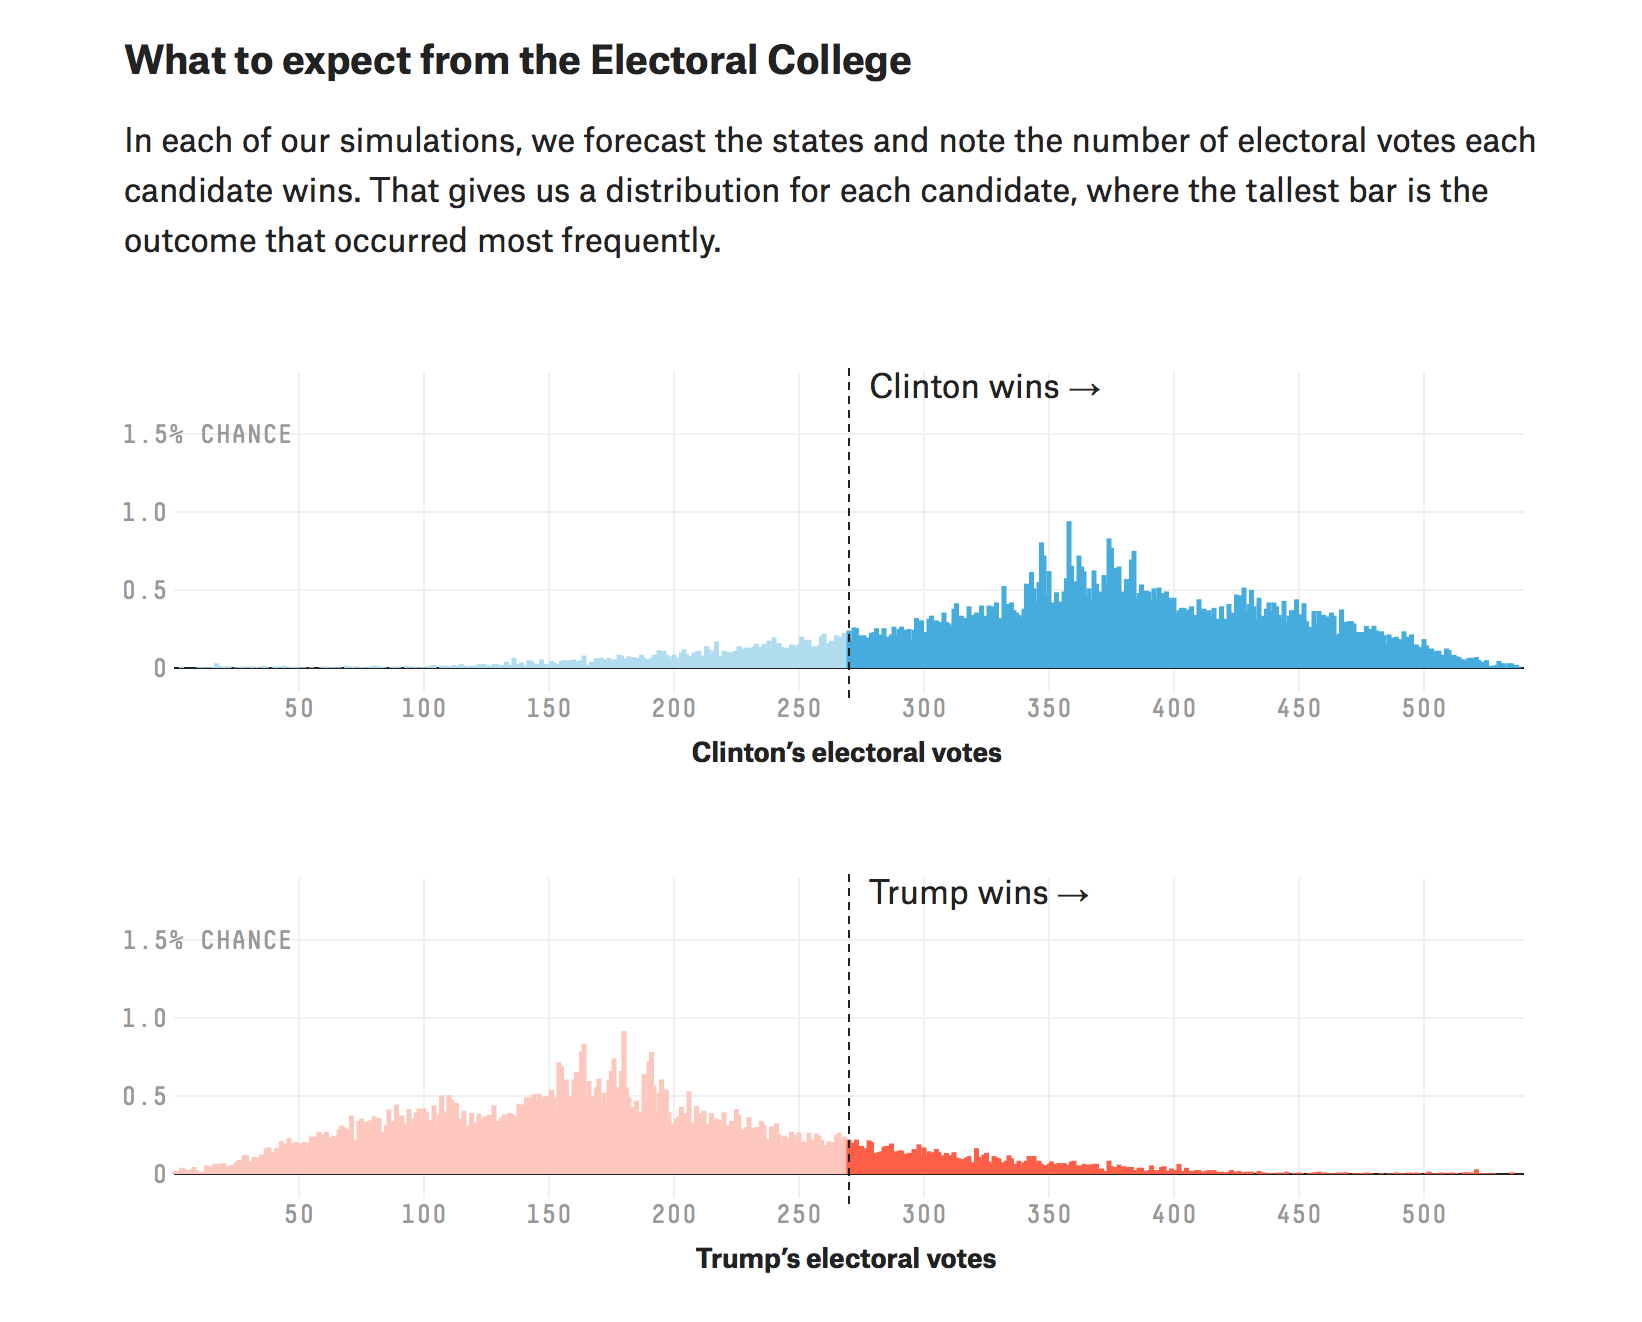
\includegraphics[scale=.5]{HillzPosteriorsYo.png}
\end{center}

\newpage

\section*{Problem}

\begin{enumerate}
\item Write out the DAG and joint distribution for this problem.

\ifanswers
\begin{center}
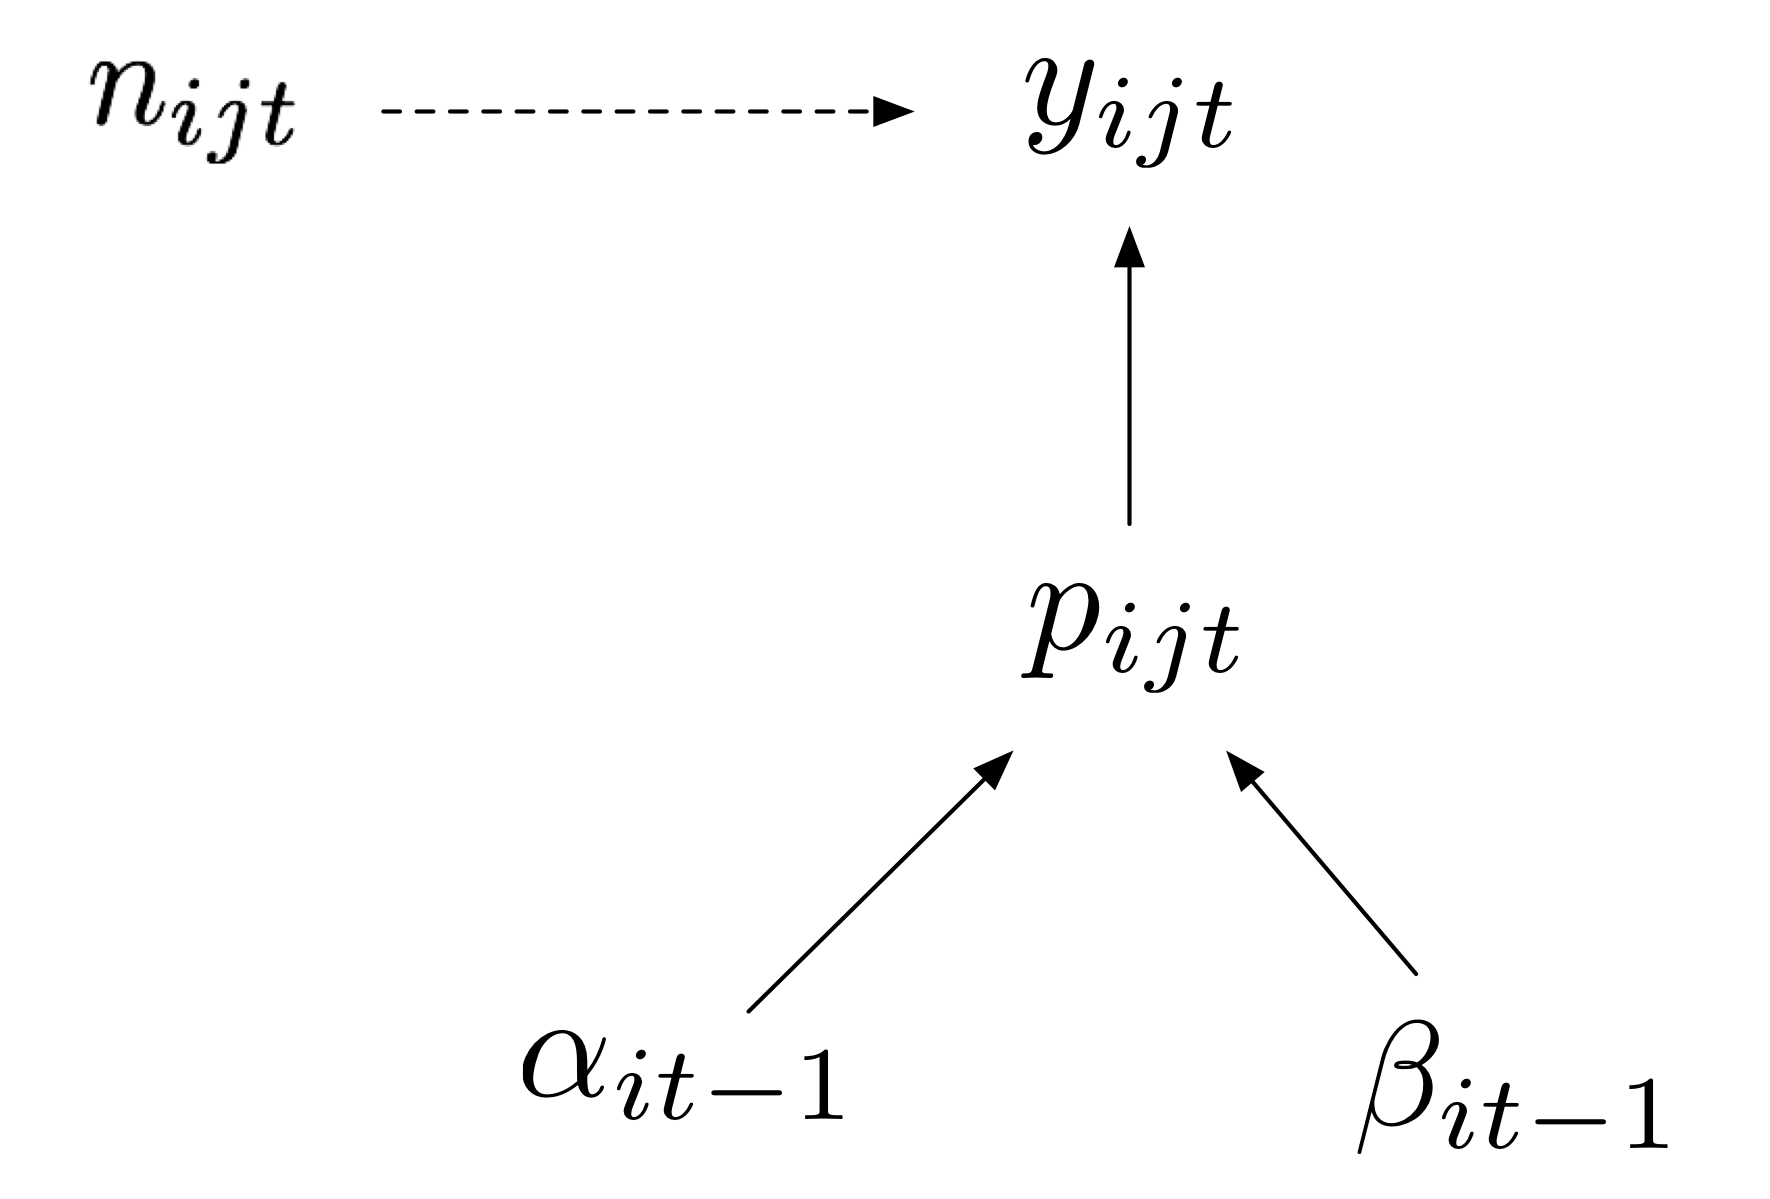
\includegraphics[scale=.4]{DAG}
\end{center}
\noindent where $y$ is the number of votes for Hillary Clinton, in the $j^{th}$ poll, in week $t$, in the $i^{th}$ state.
\begin{eqnarray*}
\big[\boldsymbol{\alpha},\boldsymbol{\beta}, \mathbf{p} \mid \mathbf{y}\big] \propto & \prod_{i=1}^{51}\prod_{j=1}^{N_{j}}\prod_{t=1}^{T} \big[y_{ijt} \mid p_{ijt}\big]\big[p_{ijt} \mid \alpha_{it},\beta_{it}\big]
\big[\alpha_{it}\big]\big[\beta_{it}\big]
\end{eqnarray*}
\fi 

\item How would you decide who wins each state? Who wins the national vote? Remember candidates must accumulate 270 of 538 state-level electoral votes to win the election.

\ifanswers
\begin{center}

$\phi_{it}=\cfrac{\alpha_{it}}{\alpha_{it}+\beta_{it}}$
\vspace{5mm}

$V_{it} = \textrm{binomial}\big(N_{it}, \phi_{it}\big)$

where $N_{it}$ is the number of likely voters in the $i^{th}$ state and the $t^{th}$ week.

if $V_{it} > \frac{N}{2}$ then $Z_{it}=1$ else $Z_{it}=0$

$E_{t} = Z_{it} \times$ the number of electoral votes $= \Sigma_{i=1}^{51} E_{it}$

$H=1$ if $E_{it} \geq 270$, then Clinton wins.

$H=0$ if $E_{it} < 270$, then Trump wins.
\end{center}
\fi

\item As the election season progresses, there is more and more information to use to inform priors.  Think about how might you incorporate a weight, $w$, for each of the priors.  We will discuss this as a group.
\vspace{-5mm}
\ifanswers
\begin{eqnarray*}
\alpha_{it} &= \Sigma^J_{j=1} w_{ij} a_{ijt-1}\\
\beta_{it} &= \Sigma^J_{j=1} w_{ij} b_{ijt-1}
\end{eqnarray*}
\fi
\end{enumerate}
\end{document}

